\begin{frame}{Motivation}
    \begin{itemize}
        \item We have seen an SPA attack on RSA implementations that exploits the part of the square and multiply algorithm that multiplication is carried out only when the secret key bit is $1$.
      \item A natural countermeasure is that we always compute multiplication no matter what the value of the secret key bit.
      \item Such an algorithm is called \textit{square and multiply-always algorithm}
    \end{itemize}
\end{frame}

\begin{frame}{RSA}
\begin{definition}[RSA]
Let $n=pq$, where $p,q$ are distinct prime numbers.
Let $\mathcal{P}=\mathcal{C}=\ZZ_n$, $\mathcal{K}=\ZZ_{\varphi(n)}^*-\Set{1}$.
For any $e\in \mathcal{K}$, define encryption
\[
    E_e:\ZZ_n\to\ZZ_n,\quad m\mapsto m^e\mo n,
\]
and the corresponding decryption
\[
    D_d:\ZZ_n\to\ZZ_n,\quad c\mapsto c^d\mo n,
\]
where $de\mo\varphi(n)=1$.
The cryptosystem $(\mathcal{P},\mathcal{C},\mathcal{K},\mathcal{E},\mathcal{D})$, where $\mathcal{E}=\Set{E_e:e\in\mathcal{K}}$, $\mathcal{D}=\Set{D_d:d\in\mathcal{K}}$, is called \textit{RSA}.
\end{definition}
\begin{itemize}
    \item $\varphi(n)=(p-1)(q-1)$
    \item Public key: $n,e$, RSA modulus, encryption exponent
    \item Private key: $d$, decryption exponent
\end{itemize}
\end{frame}

\begin{frame}{Square and multiply algorithm}
    \begin{itemize}
        \item Let $n\geq2$ be an integer, $d\in\ZZ_{\varphi(n)}^{*}$, $a\in\ZZ_n$
        \item Binary representation of $d=d_{\ell_d-1}\dots d_2d_1d_0$, where $d_i=0,1$ and
\[
d=\sum_{i=0}^{\ell_d-1}d_i2^i,
\]
\item Then we have
\[
a^d=a^{\sum_{i=0}^{\ell_d-1}d_i2^i}=\prod_{i=0}^{\ell_d-1}(a^{2^i})^{d_i}=\prod_{0\leq i<\ell_d,d_i=1}a^{2^i}.
\]
Thus, to compute $a^d\mo n$, we can 
\begin{itemize}
    \item first compute $a^{2^i}$ for $0\leq i<\ell_d$
    \item then $a^d$ is a product of $a^{2^i}$ for which $d_i=1$
\end{itemize}
    \end{itemize}
\end{frame}

\begin{frame}{Square and multiply algorithms}
\begin{columns}[T] % align columns
\begin{column}{.5\textwidth}
\begin{algorithm}[H]
\KwIn{$n,\ a,\ d$\tcp{$n\in\ZZ, n\geq2$; $a\in\ZZ_n$; $d\in\ZZ_{\varphi(n)}$ has bit length $\ell_d$}}
\KwOut{$a^d\mo n$}
result $= 1$, $t = a$\\
	\For{$i=0$, $i<\ell_d$, $i++$}
 	{
 	\tcp{$i$th bit of $d$ is $1$}
  		\If{$d_i=1$}{
            \tcp{mutiply by $a^{2^i}$}
  		$\text{result} = \text{result}*t\mo n$\tcp{$
a^d=\displaystyle\prod_{0\leq i<\ell_d,d_i=1}a^{2^i}$}
  		}
  		\tcp{$t=a^{2^{i+1}}$}
  		$t=t*t\mo n$\\
  	}
  	\Return result\\
	\caption{Right-to-left}
\end{algorithm}
\end{column}%
\hfill%
\begin{column}{.5\textwidth}
 \begin{algorithm}[H]
\KwIn{$n,\ a,\ d$\tcp{$n\in\ZZ, n\geq2$; $a\in\ZZ_n$; $d\in\ZZ_{\varphi(n)}$}}
\KwOut{$a^d\mo n$}
$t = 1$\\
	\For{$i=\ell_d-1$, $i\geq0$, $i--$}
 	{
  	$t=t*t\mo n$\\
 	\tcp{$i$th bit of $d$ is $1$}
  		\If{$d_i=1$}{
  		$t = a*t\mo n$
  		}
  	}
  	\Return t
\caption{Left-to-right}
\end{algorithm}
\end{column}%
\end{columns}
\end{frame}


\begin{frame}{Right-to-left square and multiply-always}
\begin{columns}[T] % align columns
\begin{column}{.5\textwidth}
{
\setlength{\interspacetitleruled}{0pt}%
\setlength{\algotitleheightrule}{0pt}%
\begin{algorithm}[H]
\KwIn{$n,\ a,\ d$\tcp{$n\in\ZZ, n\geq2$; $a\in\ZZ_n$; $d\in\ZZ_{\varphi(n)}$ has bit length $\ell_d$}}
\KwOut{$a^d\mo n$}
result $= 1$, $t = a$\\
	\For{$i=0$, $i<\ell_d$, $i++$}
 	{
 	\tcp{$i$th bit of $d$ is $1$}
  		\If{$d_i=1$}{
            \tcp{mutiply by $a^{2^i}$}
  		$\text{result} = \text{result}*t\mo n$\tcp{$
a^d=\displaystyle\prod_{0\leq i<\ell_d,d_i=1}a^{2^i}$}
  		}
  		\tcp{$t=a^{2^{i+1}}$}
  		$t=t*t\mo n$\\
  	}
  	\Return result\\
\end{algorithm}
}
\end{column}%
\begin{column}{.55\textwidth}
{\small
 \begin{algorithm}[H]
\KwIn{$n,\ a,\ d$
}
\KwOut{$a^d\mo n$}
result $= 1$, $t = a$\\
	\For{$i=0$, $i<\ell_d$, $i++$}
 	{
 	\tcp{$i$th bit of $d$ is $1$}
  		\If{$d_i=1$}{
            \tcp{mutiply by $a^{2^i}$}
  		$\text{result} = \text{result}*t\mo n$\\
  		}
            \Else{
            \tcp{compute multiplication and discard the result}
            $\text{tmp}=\text{result}*t\mo n$
            }
  		\tcp{$t=a^{2^{i+1}}$}
  		$t=t*t\mo n$\\
  	}
  	\Return result
	\caption{Square and multiply-always}
\end{algorithm}}
\end{column}%
\end{columns}
\end{frame}

\begin{frame}{Left-to-right square and multiply-always}
    \begin{columns}[T] % align columns
\begin{column}{.5\textwidth}
{
\setlength{\interspacetitleruled}{0pt}%
\setlength{\algotitleheightrule}{0pt}%
\begin{algorithm}[H]
\KwIn{$n,\ a,\ d$\tcp{$n\in\ZZ, n\geq2$; $a\in\ZZ_n$; $d\in\ZZ_{\varphi(n)}$ has bit length $\ell_d$}}
\KwOut{$a^d\mo n$}
$t = 1$\\
	\For{$i=\ell_d-1$, $i\geq0$, $i--$}
 	{
  	$t=t*t\mo n$\\
 	\tcp{$i$th bit of $d$ is $1$}
  		\If{$d_i=1$}{
  		$t = a*t\mo n$
  		}
  	}
  	\Return t
\end{algorithm}
}
\end{column}%
\begin{column}{.55\textwidth}
{\small
 \begin{algorithm}[H]
\KwIn{$n,\ a,\ d$
}
\KwOut{$a^d\mo n$}
$t = 1$\\
	\For{$i=\ell_d-1$, $i\geq0$, $i--$}
 	{
  	$t=t*t\mo n$\\
 	\tcp{$i$th bit of $d$ is $1$}
  		\If{$d_i=1$}{
  		$t = a*t\mo n$
  		}
            \Else{
            \tcp{$i$th bit of $d$ is $0$, compute multiplication and discard the result}
            $\text{tmp}=a*t\mo n$
            }
  	}
  	\Return t
	\caption{Square and multiply-always}
\end{algorithm}}
\end{column}%
\end{columns}
\end{frame}

\begin{frame}{SPA on left-to-right square and multiply algorithm}
For our experiment, we have set
        \[
        p=29,\quad q=41,\quad n=1189,\quad \varphi(n)=1120,\quad e=3,\quad d=747
        \]
{\small
\begin{algorithm}[H]
\KwIn{$a$\tcp{$a\in\ZZ_{1189}$}}
\KwOut{$a^{747}\mo 1189$}
$n=1189$\\
$dbin=[1,1,0,1,0,1,1,1,0,1]$\tcp{binary representation of $d=747$, $d_0=1$, $d_1=1$}
$\ell_d=\text{length of }dbin$\tcp{bit length of $d$}
$t = 1$\\
	\For{$i=\ell_d-1$, $i\geq0$, $i--$}
 	{
  	$t=t*t\mo n$\\
 	\tcp{$i$th bit of $d$ is $1$}
  		\If{$d_i=1$}{
  		$t = a*t\mo n$
  		}
  	}
  	\Return t
\caption{Left-to-right square and multiply algorithm for computing modular exponentiation with parameters from above.}
\end{algorithm}}
\end{frame}

\begin{frame}{SPA on left-to-right square and multiply algorithm}
    \begin{figure}[H]
    \centering
    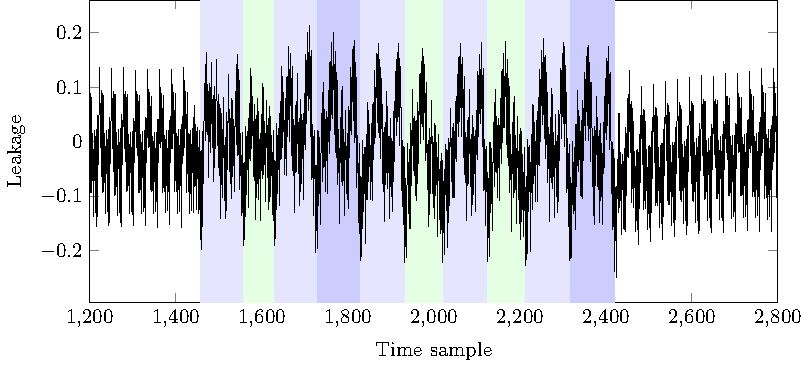
\includegraphics[width=0.9\textwidth]{fig/SPA_on_RSA_highlighted_peaks.pdf}
    \caption{Green patterns (single peak cluster) $\rightarrow$ $d_i=0$; blue patterns (multiple peak clusters) $\rightarrow$ $d_i=1$}
\end{figure}
We can read out the value of bits $d_i$: $d=1011101011=747$
\end{frame}

\begin{frame}{Implementation with countermeasure}
\[
        p=29,\quad q=41,\quad n=1189,\quad \varphi(n)=1120,\quad e=3,\quad d=747
        \]
{\small
    \begin{algorithm}[H]
\KwIn{$a$\tcp{$a\in\ZZ_{1189}$}}
\KwOut{$a^{747}\mo 1189$}
$n=1189$\\
$dbin=[1,1,0,1,0,1,1,1,0,1]$\tcp{binary representation of $d=747$, $d_0=1$, $d_1=1$}
$\ell_d=\text{length of }dbin$\tcp{bit length of $d$}
$t = 1$\\
	\For{$i=\ell_d-1$, $i\geq0$, $i--$\label{line:alg:SCA-RSA-implementation-counter:loop}}
 	{
  	$t=t*t\mo n$\label{line:alg:SCA-RSA-implementation-counter:tt}\\
 	% \tcp{$i$th bit of $d$ is $1$}
  		\If{$d_i=1$}{
  		$t = a*t\mo n$\label{line:alg:SCA-RSA-implementation-counter:at}
  		}
    \Else{
     \tcp{$i$th bit of $d$ is $0$, compute multiplication and discard the result}
            $\text{tmp}=a*t\mo n$\label{line:alg:SCA-RSA-implementation-counter:tmp}
    }
  	}
  	\Return t
\caption{
Left-to-right square and multiply-always algorithm.}
\end{algorithm}}
\end{frame}

\begin{frame}{The power trace}
    \begin{figure}[htb]
    \centering
    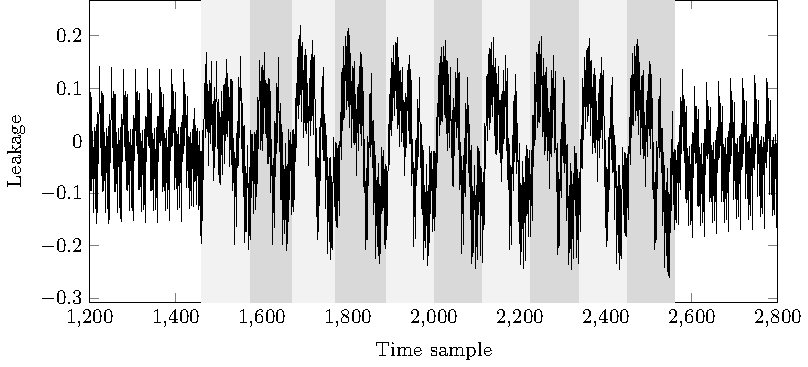
\includegraphics{fig/SPA_on_RSA_countermeasure}
    \caption{One trace corresponding to the computation of left-to-right square and multiply-always algorithm.
    We can see ten similar patterns.
    But in this case, all of them have more than one peak cluster.}
\end{figure}
\end{frame}

\begin{frame}{Comparison}
\begin{figure}[H]
    \centering
    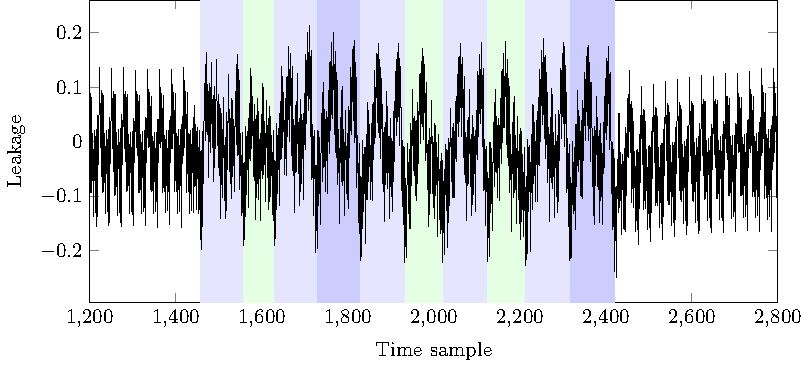
\includegraphics[width=0.6\textwidth]{fig/SPA_on_RSA_highlighted_peaks.pdf}
\end{figure}
    \begin{figure}[H]
    \centering
    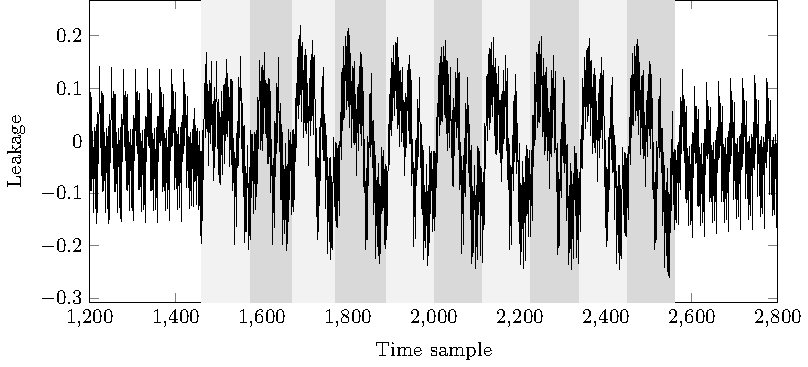
\includegraphics[width=0.6\textwidth]{fig/SPA_on_RSA_countermeasure}
\end{figure}
\end{frame}